\section{Environment Representation}
\label{sec:mapf-representation}
\hspace{\parindent}
Although MRPP can be described independently of a specific environment representation, practical
planning methods require a concrete state space in which robot motion and conflicts can be
evaluated. In multi-robot planning literature, different representations have been adopted,
primarily differing in how space and time are modeled and in the resulting level of abstraction.

Common approaches include discrete representations, such as grids and graphs, where robots occupy
a finite set of states and move between neighboring states in discrete time steps, as well as
continuous formulations, where robot motion is described by continuous trajectories and conflicts
arise from geometric interactions. Figure~\ref{fig:env_representations} illustrates how the same
workspace can be modeled under different discrete representations.

While continuous formulations offer higher modeling fidelity, discrete representations are widely
used in classical MAPF and MRPP settings due to their simplicity and structured abstraction. In this
dissertation, the focus is placed on grid and graph representations, with particular emphasis on
graph representations because the considered fleet coordination framework performs planning over a
shared roadmap.

\begin{figure}[H]
    \centering
    \begin{subfigure}{0.30\linewidth}
        \centering
        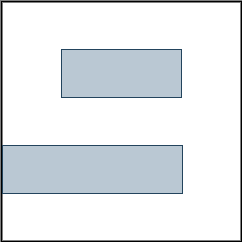
\includegraphics[width=\linewidth]{original_ground.png}
        \caption{Workspace layout}
    \end{subfigure}
    \hspace{0.5em}
    \begin{subfigure}{0.30\linewidth}
        \centering
        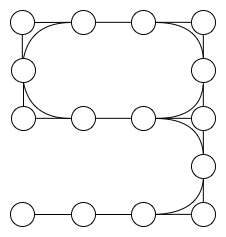
\includegraphics[width=\linewidth]{graph.png}
        \caption{Graph representation}
    \end{subfigure}
    \hspace{0.5em}
    \begin{subfigure}{0.30\linewidth}
        \centering
        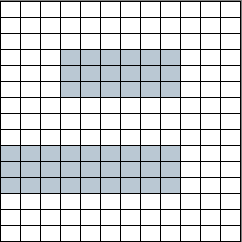
\includegraphics[width=\linewidth]{grid.png}
        \caption{Grid representation}
    \end{subfigure}

    \caption{Illustration of different discrete environment representations for the same workspace.}
    \label{fig:env_representations}
\end{figure}


\subsection{Grid Representation}
\label{subsec:grid_representation}
\hspace{\parindent}
In grid formulations, the environment is discretized into a regular two or three-dimensional array
of uniformly sized cells, each classified as free or occupied. Robots move between neighboring
cells according to a fixed connectivity structure, yielding a simple and intuitive abstraction that
has been widely adopted in early MAPF studies
\cite{yang2010grid,stern2019definitions}.

A key advantage of grid representations is their simplicity and direct correspondence to occupancy
grids used in robotic perception. However, grid resolution introduces an inherent trade-off. Coarse
grids may fail to capture narrow passages or thin obstacles, while fine grids incur substantial memory
and computational costs \cite{yang2010grid,ma2022graph}. In addition, the discrete nature of grid
motion complicates the integration of continuous-time dynamics, often requiring post-processing to
obtain executable trajectories \cite{ma2022graph}.

For these reasons, graph representations are particularly relevant in this dissertation, since the
considered fleet coordination framework performs planning over a shared roadmap~\cite{matos2025criis}. By allowing
arbitrary topologies and connectivity patterns, graph representations provide a convenient
abstraction for modeling structured environments and for supporting centralized coordination.


\subsection{Graph Representation}
\hspace{\parindent}
In graph formulations the environment is modeled as a discrete graph that
captures admissible robot states and their connectivity. This follows the modeling approach
described by Stern et al.~\cite{stern2019definitions}, while being interpreted here in the context of
multi-robot fleet coordination.

Formally, the environment is represented as a graph \(G = (V, E)\), where each vertex
\(v \in V\) corresponds to a valid state that a robot may occupy, and each edge \((u,v) \in E\)
encodes a feasible transition between states. The graph may be directed or undirected, depending on
the characteristics of the environment and on the motion constraints imposed by the planning system.

Under this representation, robot trajectories evolve in discrete time steps and are constrained to
lie on the graph. Each state \(p_i^t\) therefore corresponds to a vertex in \(V\), and successive
states satisfy
\[
p_i^{t+1} = p_i^t
\quad \text{or} \quad
(p_i^t, p_i^{t+1}) \in E.
\]
The first case represents a waiting action, while the second represents a
movement between two connected vertices~\cite{yu2013planning}.


\subsubsection{Graph Construction Approaches}
\hspace{\parindent}
Several classical approaches have been proposed to construct graph representations of planning
environments. These include roadmap approaches such as visibility graphs, which connect mutually
visible obstacle vertices \cite{lozano1979algorithm}, Voronoi diagram representations that
emphasize obstacle clearance \cite{aurenhammer1991voronoi}, and cell decomposition techniques that
subdivide the free space into regions whose adjacency defines a connectivity graph
\cite{latombe1991robot,choset2005principles}. Representative examples of these constructions are
illustrated in Figure~\ref{fig:classical_graph_construction}.

In this dissertation, the objective is not to compare graph construction methods, but to perform
multi-robot coordination over an existing graph representation. The underlying roadmap is therefore
assumed to be available, and the planning problem consists of computing coordinated robot
trajectories on top of this discrete abstraction.

\begin{figure}[H]
    \centering
    \begin{subfigure}{0.35\linewidth}
        \centering
        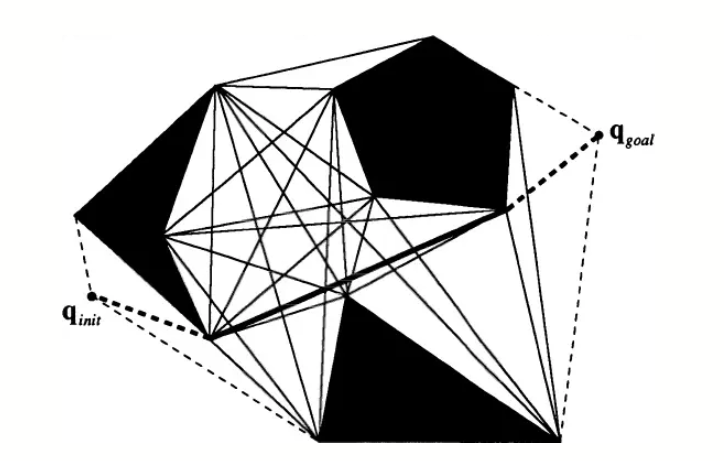
\includegraphics[width=\linewidth]{visibility_graph.png}
        \caption{Visibility graph}
    \end{subfigure}
    \hfill
    \begin{subfigure}{0.27\linewidth}
        \centering
        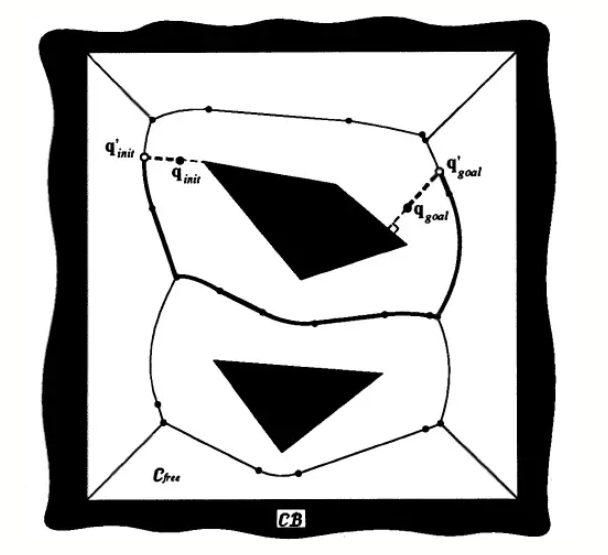
\includegraphics[width=\linewidth]{voronoi.png}
        \caption{Voronoi diagram}
    \end{subfigure}
    \hfill
    \begin{subfigure}{0.32\linewidth}
        \centering
        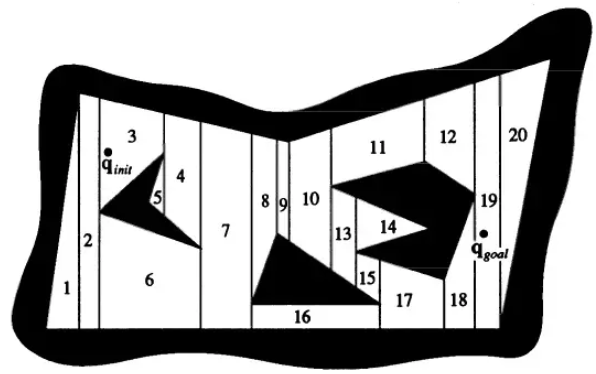
\includegraphics[width=\linewidth]{cell_decomposition.png}
        \caption{Cell decomposition}
    \end{subfigure}
    \caption{Classical approaches for constructing graph representations \cite{latombe1991robot}.}
    \label{fig:classical_graph_construction}
\end{figure}